\documentclass[conference]{IEEEtran}
\IEEEoverridecommandlockouts
% The preceding line is only needed to identify funding in the first footnote. If that is unneeded, please comment it out.
\usepackage{cite}
\usepackage{amsmath,amssymb,amsfonts}
\usepackage{algorithmic}
\usepackage{graphicx}
\usepackage[tight,footnotesize]{subfigure}
\usepackage{textcomp}
\usepackage{xcolor}

%for hungarian letters
\usepackage[utf8]{inputenc}

\def\BibTeX{{\rm B\kern-.05em{\sc i\kern-.025em b}\kern-.08em
    T\kern-.1667em\lower.7ex\hbox{E}\kern-.125emX}}


\title{Hindsight Experience Replay with Environment Relabeling \\
	\bigskip
\Large{Milestone Report}}

\author{\IEEEauthorblockN{Katharina Hermann}
	\IEEEauthorblockA{\textit{Technische Universität München}}
	\textit{Department of Informatics}
	\and
	\IEEEauthorblockN{Ferenc Török}
	\IEEEauthorblockA{\textit{Technische Universität München}}
	\textit{Department of Informatics}
}

\begin{document}
\maketitle

\begin{abstract}
	This document is written as a milestone report for the project of the subject Advanced Deep Learning in Robotics at the Technische Universität München. Our chosen topic is to develop a method to train a Reinforcement Learning \cite{sutton_barto} agent effectively to solve the task of motion planning in an environment with obstacles. The aim of the method is to reduce training time as much as possible meanwhile using a very simple reward function.
\end{abstract}

\section{Introduction}
Navigate a robot in an environment where obstacles are present, and with which the agent must not collide, is a challenging task even in the simplest cases. There are several techniques on the classical Motion Planning field, which aim to solve this problem. This methods perform well in many cases, however often times they become computationally very expensive. Also, many planning and control methods assume an exact model of the robot and the environment and perform poorly, if these requirements are not met, i.e. the environment is noisy.

Reinforcement Learning (RL) agents are although very demanding to train, later have minimal computational requirements: The evaluation of a trained model is very cheap and fast. Also, well trained agents are often resistant to noises in the environment. At last, many training methods don't even require a model of the agent nor the environment and hence inaccuracies or instabilities due to model mismatch can be avoided. The above mentioned properties make RL techniques to be appealing for motion planning. RL combined with neural networks as function approximators yield the so called Deep Reinforcement Learning (DRL), which when used for motion planning is referred to as Neural Motion Planning (NMP) \cite{NMP}.

RL agents learn by interacting with the environment and receive rewards from it. Engineering the reward function for a given task is an important and often very complicated task. There is a trade-off between reward function complexity and training efficiency. Carefully detailed reward functions are difficult to engineer, however training based on these reward functions will be quick and effective. On the other hand, creating a very sparse basic reward function is extremely low effort, however it can result in unstable and very slow training. The aim of our work is to develop a training method for training an agent to navigate in a workspace with obstacles and reach its goal with a very simple reward function. For this we are going to extend the method Hindsight Experience Replay (HER) \cite{HER} for our purposes.

\section{HER with Environment Relabeling}

If the reward function is very sparse, it can happen during training that an agent almost never receives a positive reward and hence there is no real information in the training data fed to the neural networks. To remedy this issue, \cite{HER} proposes a method to reuse unsuccessful episode trajectories by a method called relabeling. The central idea of the method is, that although this trajectory is a bad solution for the given problem, it would have been a perfectly fine trajectory for a different goal. Hence the trajectory is also saved for replay with a different goal, for which it would have been a good solution. \cite{GHER} generalizes the method not just for different goals but for different continuous reward functions.

In our project, we have the task to navigate from one point to an other in a workspace which contains some obstacles which should be avoided. Or reward function is as simple as it gets: the agent receives a reward in the amount of $+1$ if the it has reached the goal, $-1$ if it has collided with an obstacle or left the workspace and $-0.01$ after every timestep. 

To compensate for the sparsity of our reward function, we decided to use HER. However in our case, a simple goal relabeling is not enough, we also have to find a workspace with its obstacles, for which the unsuccessful trajectory poses a good solution. In this respect, the novelty in our approach is the so called Environment Relabeling, which extends HER for use cases, where the environment is not static. Here simple goal relabeling would not be enough to solve the problem of Neural Motion Planning.

\section{Experiment Setup}

\textit{Agent}: For now we have used a point-mass robot in 2D for the sake of simplicity. The robot has got a radius. If an obstacle is closer than the radius, a collision occurred. Also, if the goal is within the agent's radius, it is considered to be reached. The agent has 2 continuous actions with which it is able to interact with the environment, a x and y direction step distance. These can be arbitrary values between their respective maximum and minimum values.

\textit{Workspace}: Workspaces are represented as a $32 \times 32$ grid, where each grid cell is either free space (value $0$) or obstacle (value$1$). The number of obstacles, their position and size are generated randomly. 

\textit{Start, goal}: Start and goal positions are also generated randomly for a given workspace. A workspace with the obstacles, the goal and the agent is illustrated in Figure \ref{fig:1}.

\begin{figure}[h!]
	\centering
	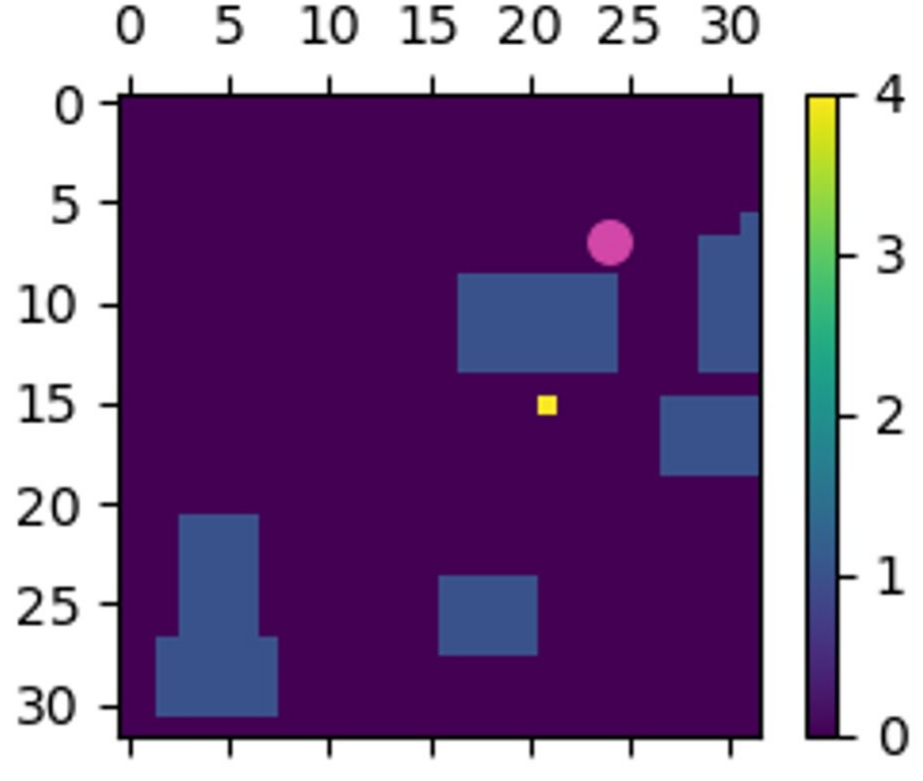
\includegraphics[width=0.2\textwidth]{fig/workspace.jpg}
	\caption{Workspace with obstacles (light blue), agent (pink) and goal (yellow)}
	\label{fig:1}
\end{figure}

\section{Implementation}

We have chosen the agent to be trained with Deep Deterministic Policy Gradient (DDPG) \cite{DDPG} which is an Actor-Critic algorithm. We use an off-the-shelf implementation, the python package TF2RL \cite{TF2RL}. This package implements various RL methods in Tensorflow 2.x. For the environment we have implemented a custom Open-AI gym environment.

The main building blocks of the project are as follows:
\begin{itemize}
	\item Workspace and goal generation.
	\item Convolutional Autoencoder (CAE) for reducing the workspace representation size. This is necessary since the workspace in its original form is represented with a feature vector of size $1024$. Compared to this, the state of the robot and the goal are represented with $2-2$ features. The workspace feature vector reduction is necessary not to loose the information about the state and goal positions.
	\item Environment implementation as a custom Open-AI gym environment.
	\item Workspace relabeling implementation
	\item Implementation of the trainer class with HER and environment relabeling.
	\item Tests
\end{itemize}

\section{Progress}

So far we have made the following progress:
\begin{itemize}
	\item Implemented and tested workspace, start and goal generation.
	\item Implemented, tested and trained the CAE on $10000$ workspaces. For the encoder we have used 3 Convolutional layers with filter sizes of $[4, 8, 16]$ followed by max-pooling for size reduction. Then after a linear layer the feature size was reduced to the latent space dimension, which is $16$. For the decoding we have used a linear layer followed by transpose convolutional and convolutional layers. We have used weighted binary cross entropy loss for training. With this method we have achieved $96\%$ accuracy on the test set. An example of the original and the output image can be seen on Figure \ref{fig:2}.
	\item Implemented and tested the custome Open-AI gym environment
	\item Implemented and tested a simple relabeling method. The method so far is very simple, it only removes the obstacle into which the agent has collided or shifts the workspace and the trajectory if the agent has left the workspace. The new goal is the last state of the trajectory.
	\item Implemented the training method with her and workspace relabeling. Testing is in progress.
\end{itemize}

\begin{figure}
	\begin{center}
		\subfigure[Input \label{fig5a}]{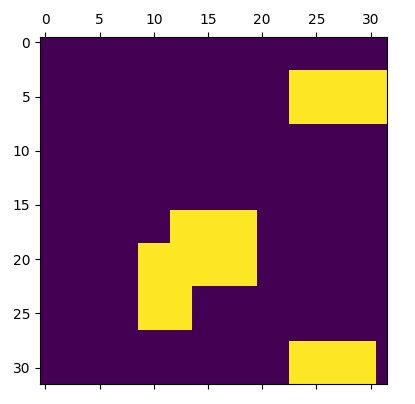
\includegraphics[width=0.2\textwidth]{fig/cae_orig.jpg}}
		~
		\subfigure[Output \label{fig5b}]{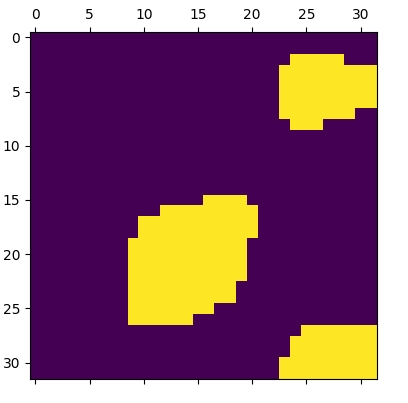
\includegraphics[width=0.196\textwidth]{fig/cae_gen.jpg}}
	\end{center}
	\vspace{-4mm}
	\caption{The input and output of the trained Convolutional Autoencoder on a test image.}
	\label{fig:2}
	\vspace{-0mm}
\end{figure}

\section{Future work}

After we finish testing the training method, we will start experimenting with the training. Hopefully after finding the sufficient hyperparameters, we will be able to train the agent successfully. Then we will analyze the results and compare it to an agent that was trained with a different method. 

If there will be enough time remaining, we will experiment with more sophisticated relabeling methods and possibly try to apply the whole method to a more complex robot, for example to a robot arm.


\bibliographystyle{IEEEtran}
\bibliography{bib/references.bib}
		
\end{document}